\documentclass[11pt]{article}
\usepackage{enumerate}
\usepackage{tikz,tikz-cd,tikz-3dplot,pgfplots}
\usepackage{amsmath,amsthm,amssymb,amsfonts,amsthm}
\usepackage{hyperref}
\usepackage{mathrsfs}
\usepackage{bm,bbm}
\usepackage{braket}
\usepackage{slashed}
\usepackage{tensor}
\usepackage{indentfirst}
\usepackage[a4paper, total={6.5in, 9in}]{geometry}
\usetikzlibrary{decorations.markings,positioning,decorations.pathmorphing}
\allowdisplaybreaks
\pgfplotsset{width=10cm, compat=1.16}
\renewcommand\bra[1]{{\langle{#1}|}}
\renewcommand\ket[1]{{|{#1}\rangle}}
\renewcommand\bfdefault{b}

\newtheorem{theorem}{Theorem}[section]
\newtheorem{lemma}[theorem]{Lemma}
\newtheorem{corollary}{Corollary}[theorem]
\theoremstyle{definition}
\newtheorem{definition}{Definition}[section]
\theoremstyle{remark}
\newtheorem{remark}{Remark}[section]

\DeclareMathOperator{\sech}{sech}
\DeclareMathOperator{\csch}{csch}
\DeclareMathOperator{\arcsec}{arcsec}
\DeclareMathOperator{\arccot}{arccot}
\DeclareMathOperator{\arccsc}{arccsc}
\DeclareMathOperator{\arccosh}{arccosh}
\DeclareMathOperator{\arcsinh}{arcsinh}
\DeclareMathOperator{\arctanh}{arctanh}
\DeclareMathOperator{\arcsech}{arcsech}
\DeclareMathOperator{\arccsch}{arccsch}
\DeclareMathOperator{\arccoth}{arccoth} 

\begin{document}
	\title{One-Loop Scheme Independence\\ \small What does complex-on-shell scheme really mean?}
	\maketitle
	\section{Basics}
	\subsection{Self energy}
	Consider a one-loop self energy calculation:
	\[\Pi(p^{2})=\frac{\alpha_{b}}{4\pi}F_{\text{loop}}(p^{2})+\delta_{Z}p^{2}-\delta_{M},\]
	where $F_{\text{loop}}$ is the result of a divergent loop integration and $\alpha_{b}$ is calculated by a bare coupling between the mother particle and loop particles.
	In a renormalised QFT, we choose the counterterms $\delta_{Z}$ and $\delta_{M}$ so that they can eliminate the infinities ($\sim\frac{1}{\epsilon}$ in dimreg) generated by loop integration.
	There is no canonical choice for those counterterms;
	We must cancel the divergent terms, however, for the finite parts, it is merely a matter of choice.
	We may separate counterterms in two parts.
	The first part only cancels the $1/\epsilon$ divergences, and the second part is remaining finite part of the counterterms:
	\[\delta_{Z}=\frac{\alpha_{b}}{4\pi}i_{Z}+f_{Z},\quad\delta_{M}=\frac{\alpha_{b}}{4\pi}i_{M}+f_{M}.\]
	Now, $F_{\text{fin}}:=F_{\text{loop}}+i_{Z}p^{2}-i_{M}$ has no $1/\epsilon$ term, so is finite unless there are other divergences such as IR divergence.
	With UV divergence canceled, we may rewrite the expression for the one-loop self energy:
	\[\Pi(p^{2})=\frac{\alpha_{b}}{4\pi}F_{\text{fin}}(p^{2})+f_{Z}p^{2}-f_{M}.\]
	In the $\mathrm{MS}$ scheme, we only cancel the divergences and nothing more, hence $f_{Z}=f_{M}=0$.
	But in the other schemes, they are generally not zero.
	
	\subsection{Propagator and pole mass}
	The one-loop corrected propagator is
	\[\frac{Z}{p^{2}-M_{b}^{2}+\Pi(p^{2})},\]
	where $M_{b}$ is a bare mass parameter of the mother particle.
	Generally $M_{b}$ is not a physical mass of the particle, so it is desirable to mention which renormalisation scheme we are working on.
	So I will notate the scheme on the mass parameter (e.g. $M_{\mathrm{MS}}$) if we work in the specific scheme.
	
	Until now, every parameters were not physical.
	The only physical mass is the pole mass $\mu$, which is defined by the position of pole of the propagator:
	\[\mu^{2}-M_{b}^{2}+\Pi(\mu^{2})=0.\]
	Using this equation, we can find $\mu$ if we fixed the scheme and given the model parameters such as $M_{b}$ and $\alpha_{b}$.
	If $\mu$ is complex then we may write $\mu=M-\frac{i}{2}\Gamma$, where $M$ is a real physical mass of the mother particle and $\Gamma$ is a decay width. (citation needed)
	
	\section{Complex-on-shell scheme}
	\subsection{Bridge between different schemes}
	Suppose that two researchers, Alice and Bob, are examining the same process.
	However, they are using different scheme, thus they have two different expressions for the propagator:
	\[\Delta_{A}(p^{2})=\frac{Z_{A}}{p^{2}-M_{A}^{2}+\Pi_{A}(p^{2})},\quad\Delta_{B}(p^{2})=\frac{Z_{B}}{p^{2}-M_{B}^{2}+\Pi_{B}(p^{2})},\]
	where the self-energies are
	\[\Pi_{A}(p^{2})=\frac{\alpha_{A}}{4\pi}F_{\text{fin}}(p^{2})+f_{Z;A}p^{2}-f_{M;A},\quad\Pi_{B}(p^{2})=\frac{\alpha_{B}}{4\pi}F_{\text{fin}}(p^{2})+f_{Z;B}p^{2}-f_{M;B}.\]
	Since they are describing the same physical process, the pole mass has to be the same:
	\[\mu^{2}-M_{A}^{2}+\Pi_{A}(\mu^{2})=\mu^{2}-M_{B}^{2}+\Pi_{B}(\mu^{2})=0,\]
	so $M_{A}^{2}=\mu^{2}+\Pi_{A}(\mu^{2})$ and $M_{B}^{2}=\mu^{2}+\Pi_{B}(\mu^{2})$.
	Expanding $\Pi(p^{2})$, we get
	\begin{align*}
		0&=\mu^{2}-M_{A}^{2}+\Pi_{A}(\mu^{2})\\
		&=(1+f_{Z;A})\mu^{2}-M_{A}^{2}+\frac{\alpha_{A}}{4\pi}F_{\text{fin}}(\mu^{2})-f_{M;A},
	\end{align*}
	and the similar equation holds for $B$.
	If we assume that the (scheme-dependent) model parameters $\alpha_{b}$, $M_{b}$, $f_{Z}$, and $f_{M}$ are real, then we can take imaginary part on the RHS and get
	\[(1+f_{Z;A})\mathrm{Im}[\mu^{2}]+\frac{\alpha_{A}}{4\pi}\mathrm{Im}[F_{\text{fin}}(\mu^{2})]=(1+f_{Z;B})\mathrm{Im}[\mu^{2}]+\frac{\alpha_{B}}{4\pi}\mathrm{Im}[F_{\text{fin}}(\mu^{2})]=0.\]
	Therefore,
	\begin{align*}
		p^{2}+\Pi_{A}(p^{2})-M_{A}^{2}&=p^{2}+\Pi_{A}(p^{2})-\mu^{2}-\Pi_{A}(\mu^{2})\\
		&=(1+f_{Z;A})(p^{2}-\mu^{2})+\frac{\alpha_{A}}{4\pi}[F_{\text{fin}}(p^{2})-F_{\text{fin}}(\mu^{2})]\\
		&=\frac{\alpha_{A}}{4\pi}\left[-\frac{\mathrm{Im}[F_{\text{fin}}(\mu^{2})]}{\mathrm{Im}[\mu^{2}]}(p^{2}-\mu^{2})+F_{\text{fin}}(p^{2})-F_{\text{fin}}(\mu^{2})\right].
	\end{align*}
	This clearly shows that
	\[\frac{\alpha_{A}}{4\pi Z_{A}}\Delta_{A}(p^{2})=\frac{\alpha_{B}}{4\pi Z_{B}}\Delta_{B}(p^{2})=\frac{1}{-\frac{\mathrm{Im}[F_{\text{fin}}(\mu^{2})]}{\mathrm{Im}[\mu^{2}]}(p^{2}-\mu^{2})+F_{\text{fin}}(p^{2})-F_{\text{fin}}(\mu^{2})}.\]
	Indeed, although their model parameters are scheme-dependent, their propagators are the same up to multiplicative factor.
	
	\subsection{Complex-on-shell scheme}
	Our third researcher, Chris, is trying to fix the form of a propagator only given the pole mass $\mu$.
	He focuses to the result of the previous chapter,
	\[\frac{\alpha_{A}}{4\pi Z_{A}}\Delta_{A}(p^{2})=\frac{\alpha_{B}}{4\pi Z_{B}}\Delta_{B}(p^{2})=\frac{1}{-\frac{\mathrm{Im}[F_{\text{fin}}(\mu^{2})]}{\mathrm{Im}[\mu^{2}]}(p^{2}-\mu^{2})+F_{\text{fin}}(p^{2})-F_{\text{fin}}(\mu^{2})}.\]
	The RHS is totally determined by $\mu$ and $F_{\text{fin}}$, and we showed that it doesn't contain any scheme-dependent parameters.
	This is a good news, but we have to determine the total multiplicative factor to define $\Delta_{C}(p^{2})$.
	Chris wants to compare his result with the Breit-Wigner distribution,
	\[D_{BW}(p^{2})=\left|\frac{1}{p^{2}-\mu^{2}}\right|^{2}.\]
	If Chris' expression for the propagator is
	\[\Delta_{C}(p^{2})=\frac{k}{-\frac{\mathrm{Im}[F_{\text{fin}}(\mu^{2})]}{\mathrm{Im}[\mu^{2}]}(p^{2}-\mu^{2})+F_{\text{fin}}(p^{2})-F_{\text{fin}}(\mu^{2})}\]
	for a real $k$ then near $p^{2}=\mu^{2}$,
	\[|\Delta_{C}(p^{2})|^{2}\approx k^{2}\left|\frac{1}{p^{2}-\mu^{2}}\right|^{2}\left|\frac{1}{-\frac{\mathrm{Im}[F_{\text{fin}}(\mu^{2})]}{\mathrm{Im}[\mu^{2}]}+F_{\text{fin}}'(\mu^{2})}\right|^{2}.\]
	Hence, if we require that $|\Delta_{C}(p^{2})|^{2}\approx D_{BW}(p^{2})$ near the pole then
	\[k=\left|-\frac{\mathrm{Im}[F_{\text{fin}}(\mu^{2})]}{\mathrm{Im}[\mu^{2}]}+F_{\text{fin}}'(\mu^{2})\right|.\]
	Therefore, Chris finally obtains
	\[\Delta_{C}(p^{2})=\frac{\left|-\frac{\mathrm{Im}[F_{\text{fin}}(\mu^{2})]}{\mathrm{Im}[\mu^{2}]}+F_{\text{fin}}'(\mu^{2})\right|}{-\frac{\mathrm{Im}[F_{\text{fin}}(\mu^{2})]}{\mathrm{Im}[\mu^{2}]}(p^{2}-\mu^{2})+F_{\text{fin}}(p^{2})-F_{\text{fin}}(\mu^{2})}=\frac{\left|1-\frac{\mathrm{Im}[\mu^{2}]}{\mathrm{Im}[F_{\text{fin}}(\mu^{2})]}F_{\text{fin}}'(\mu^{2})\right|}{p^{2}-\mu^{2}-\frac{\mathrm{Im}[\mu^{2}]}{\mathrm{Im}[F_{\text{fin}}(\mu^{2})]}[F_{\text{fin}}(p^{2})-F_{\text{fin}}(\mu^{2})]}.\]
	Looking at the RHS, it seems like we are using the complex pole mass $\mu$ in place of $M_{b}$.
	Also, the factor $-\frac{\mathrm{Im}[\mu^{2}]}{\mathrm{Im}[F_{\text{fin}}(\mu^{2})]}$ is taking a role of coupling $\alpha_{b}$ and $F_{\text{fin}}(\mu^{2})$ is taking a role of the finite part of the counterterm.
	For a stable particle, the on-shell scheme uses the real pole mass $M$ as a mass parameter, so $M_{\mathrm{OS}}=M$.
	For this reason, we may call Chris' scheme the \textbf{complex-on-shell scheme} ($\mathrm{COS}$).
	
	\subsection{Additional justifications}
	One may question, why aren't the coupling $\alpha$ showing in the COS scheme?
	That is because $\mu$ and $\alpha$ is not completely independent.
	Let $a$ be the mother particle and $b$ is a two-particles state which appears in the loop, so we are dealing with $a\to b\to a$ loop process.
	If we try to measure the $a-b$ coupling constant $\alpha$, then we may observe the decay process $a\to b$ and measure the decay width $\Gamma(a\to b)$ to determine $\alpha$.
	However, that decay width $\Gamma(a\to b)$ is precisely the width $\Gamma$ showing in the complex pole $\mu=M-\frac{i}{2}\Gamma$.
	Therefore, we expect the relation $\alpha\propto\Gamma=-\frac{1}{m}\mathrm{Im}[\mu^{2}]$.
	(For stable particles, there is no decay width to be fixed so we do not have this issue.)
	
	To put it another way, in the $\mathrm{MS}$ or $\overline{\mathrm{MS}}$ scheme, there are two degrees of freedom ($M_{b}$ and $\alpha_{b}$) for the model parameters.
	If we fix $\mu$, then it already has two degrees of freedom ($M$ and $\Gamma$), so there should be no additional free parameters.
	
	\section{Example: scalar loop}
	We take a massive real scalar particle as a mother particle and a complex real scalar with mass $m=0.45\,\mathrm{GeV}$ as a loop particle.
	One-loop calculation gives
	\[\Pi_{\overline{\mathrm{MS}}}(p^{2})=\frac{g^{2}}{16\pi^{2}}\int_{0}^{1}dx\,\ln\frac{\nu^{2}}{-x(1-x)p^{2}+m^{2}}\]
	for a fixed $\overline{\mathrm{MS}}$ reference scale $\nu$.
	We will investigate three different scheme describing the same physics (same pole mass).
	Especially, we fix $\mu=1\,\mathrm{GeV}-\frac{i}{2}0.2\,\mathrm{GeV}$.
	
	Our first scheme is $\overline{\mathrm{MS}}$ scheme.
	Taking $\nu=1\,\mathrm{GeV}$, we must have $M_{\overline{\mathrm{MS}}}=1.172\,\mathrm{GeV}$ and $g_{\overline{\mathrm{MS}}}=4.066\,\mathrm{GeV}$ so that the pole mass $\mu$ can be the value we fixed.
	
	The next scheme is real-on-shell scheme, where we require $\mathrm{Re}[\Pi_{\mathrm{OS}}(M_{\mathrm{OS}}^{2})]=0$ and $\mathrm{Re}[\Pi_{\mathrm{OS}}'(M_{\mathrm{OS}}^{2})]=0$.
	Hence, the self-energy takes the form of
	\begin{align*}
		\Pi_{\mathrm{OS}}(p^{2})=\frac{g^{2}}{16\pi^{2}}\bigg(&\int_{0}^{1}dx\,\left[\ln\frac{1}{-x(1-x)p^{2}+m^{2}}-\ln\left|\frac{1}{-x(1-x)M_{\mathrm{OS}}^{2}+m^{2}}\right|\right]\\
		&-(p^{2}-M_{\mathrm{OS}}^{2})\int_{0}^{1}dx\,\frac{x(1-x)}{x(1-x)M_{\mathrm{OS}}^{2}-m^{2}}\bigg).
	\end{align*}
	Also the on-shell mass and couplings are $M_{\mathrm{OS}}=1.024\,\mathrm{GeV}$ and $g_{\mathrm{OS}}=4.500\,\mathrm{GeV}$ to match the location of complex pole.
	
	The last scheme is $\mathrm{COS}$ scheme.
	Here we take
	\[F_{\mathrm{fin}}=\int_{0}^{1}dx\,\ln\frac{\nu^{2}}{-x(1-x)p^{2}+m^{2}}.\]
	It seems like the arbitrary parameter $\nu$ is presenting, but it actually cancels out in the final expression.
	
	We plot the resonance shapes for three schemes in Figure \ref{fig:3scheme}.
	For the $\mathrm{COS}$ scheme, we plotted $|\Delta_{C}(p^{2})|^{2}$, and for the rest, we plotted $|p^{2}-M^{2}+\Pi(p^{2})|^{-2}$.
	We can notice that the shape looks similar.
	Indeed, if we rescale the height of the peaks so that each peak's height is equal to that of the complex-on-shell scheme (Figure \ref{fig:3scheme2}), then the graphs overlap perfectly.
	To compare, we also plotted Breit-Wigner distribution on top of them, also matching the peak height.
	
	\begin{figure}[h]
		\centering
		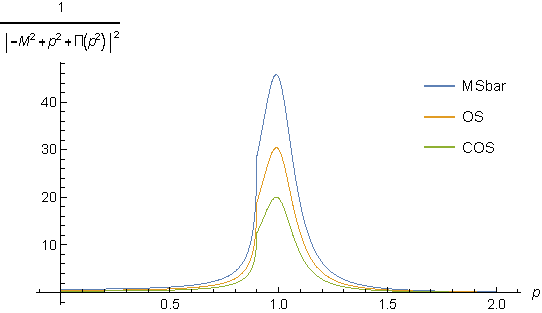
\includegraphics[width=0.6\textwidth]{olsi1.pdf}
		\caption{resonance shapes without field strength renormalisation.}
		\label{fig:3scheme}
	\end{figure}
	\begin{figure}[h]
		\centering
		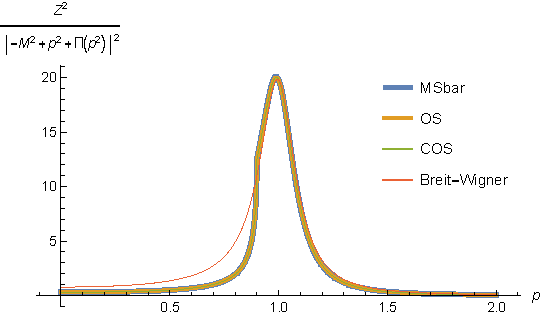
\includegraphics[width=0.6\textwidth]{olsi2.pdf}
		\caption{resonance shapes with field strength renormalisation.}
		\label{fig:3scheme2}
	\end{figure}
	
	\subsection{A faulty naive complex-on-shell scheme}
	Following the usual procedure for the on-shell renormalisation, one may be tempted to use the following `naive complex-on-shell' scheme ($\mathrm{NCOS}$):
	\[\Pi_{\mathrm{NCOS}}(\mu^{2})=0,\quad\Pi'_{\mathrm{NCOS}}(\mu^{2})=0\]
	while choosing $\mu$ and $\alpha_{\mathrm{NOS}}$ freely.
	Then the self-energy is
	\begin{align*}
		\Pi_{\mathrm{NCOS}}(p^{2})=\frac{g^{2}}{16\pi^{2}}\bigg(&\int_{0}^{1}dx\,\left[\ln\frac{1}{-x(1-x)p^{2}+m^{2}}-\ln\frac{1}{-x(1-x)\mu^{2}+m^{2}}\right]\\
		&-(p^{2}-\mu^{2})\int_{0}^{1}dx\,\frac{x(1-x)}{x(1-x)\mu^{2}-m^{2}}\bigg).
	\end{align*}
	This shouldn't be right, since we introduced fake degrees of freedom.
	In Figure \ref{fig:NCOS}, we can see that the $\mathrm{NCOS}$ scheme produces different resonance shape even when we match the peak height.
	
	\begin{figure}[h]
		\centering
		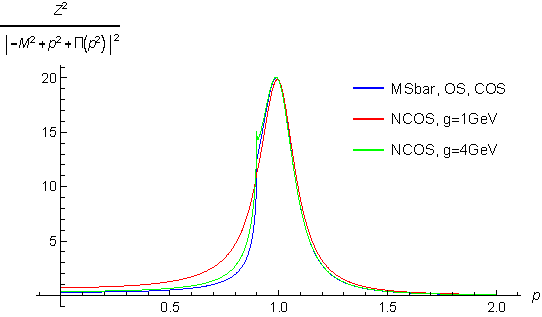
\includegraphics[width=0.6\textwidth]{olsi3.pdf}
		\caption{Naive complex-on-shell scheme cannot represent the resonance shape correctly.}
		\label{fig:NCOS}
	\end{figure}
	
	\section{Many decay channels and partial width}
	In general, there can be many decay channels for the mother particle $A$.
	That is, we have several two-particle states $B_{1},\dots,B_{N}$ so that $A$ can decay into $B_{i}$.
	This automatically means that there are loop diagrams $A\to B_{i}\to A$.
	In this case, the pole mass $\mu$ alone is not enough to parametrise the whole process;
	We need to fix either coupling constants or partial width for each processes.
	
	Again, we start with the self-energy
	\[\Pi_{b}(p^{2})=f_{Z}p^{2}-f_{M}+\sum_{i=1}^{N}\frac{\alpha_{b,i}}{4\pi}F_{\text{fin},i}(p^{2}).\]
	Then taking imaginary part of the pole equation $\mu^{2}-M_{b}^{2}+\Pi(\mu^{2})=0$ gives
	\[(1+f_{Z})\mathrm{Im}[\mu^{2}]+\sum_{i=1}^{N}\frac{\alpha_{b,i}}{4\pi}\mathrm{Im}[F_{\text{fin},i}(\mu^{2})]=0.\]
	Since $\mathrm{Im}[\mu^{2}]=-M\Gamma$, we rewrite the equation:
	\[\Gamma=\sum_{i=1}^{N}\frac{\alpha_{b,i}}{4\pi M(1+f_{Z})}\mathrm{Im}[F_{\text{fin},i}(\mu^{2})].\]
	Then it is natural to associate each summand in the RHS to partial width $\Gamma_{i}$:
	\[\Gamma_{i}:=\frac{\alpha_{b,i}}{4\pi M(1+f_{Z})}\mathrm{Im}[F_{\text{fin},i}(\mu^{2})].\]
	Then we have
	\begin{align*}
		p^{2}-M_{b}^{2}+\Pi(p^{2})&=p^{2}-\mu^{2}+\Pi(p^{2})-\Pi(\mu^{2})\\
		&=(1+f_{Z})(p^{2}-\mu^{2})+\sum_{i=1}^{N}\frac{\alpha_{b,i}}{4\pi}[F_{\text{fin},i}(p^{2})-F_{\text{fin},i}(\mu^{2})]\\
		&=(1+f_{Z})(p^{2}-\mu^{2})+\frac{(1+f_{Z})M}{\mathrm{Im}[F_{\text{fin},i}(\mu^{2})]}\sum_{i=1}^{N}\Gamma_{i}[F_{\text{fin},i}(p^{2})-F_{\text{fin},i}(\mu^{2})].
	\end{align*}
	Again, if we require that $|\Delta_{C}(p^{2})|^{2}\approx D_{BW}(p^{2})$ near the pole, then we can fix the overall scaling of the propagator and get
	\[\Delta_{C}(p^{2})=\frac{\displaystyle\left|1+\frac{M}{\mathrm{Im}[F_{\text{fin},i}(\mu^{2})]}\sum_{i=1}^{N}\Gamma_{i}[F_{\text{fin},i}'(\mu^{2})]\right|}{\displaystyle p^{2}-\mu^{2}+\frac{M}{\mathrm{Im}[F_{\text{fin},i}(\mu^{2})]}\sum_{i=1}^{N}\Gamma_{i}[F_{\text{fin},i}(p^{2})-F_{\text{fin},i}(\mu^{2})]}.\]
	We have one subtle point:
	The partial width $\Gamma_{i}$ is nonzero even if two-particle state $B_{i}$ is heavier than the real part of the pole mass $M$.
	That is because since $\mu^{2}$ is complex, $\mathrm{Im}[F_{\text{fin},i}(\mu^{2})]$ is nonzero regardless of the mass of the loop particles.
	One intuitive explanation for this would be that the unstable mother particle is never on-shell, so its (real) mass is always ambiguous.
	Thus, $A$ can decay into $B_{i}$ on the tail of its resonance.
	
	To sidestep this subtlety, we can `trust the process' and use other schemes ($\overline{\mathrm{MS}}$, $\mathrm{OS}$, etc., but not $\mathrm{NCOS}$) instead.
	Then we can explicitly fix every $\alpha_{i}$, but matching $\mu$ (so the total width) is not easy.
	
\end{document}